\documentclass{article}
\usepackage{amsmath,amssymb}
\usepackage{graphicx}
\usepackage{xcolor}
\usepackage{listings}
\renewcommand{\baselinestretch}{1.5}
\setlength{\parskip}{1em}
\definecolor{codegreen}{rgb}{0,0.6,0}
\definecolor{codegray}{rgb}{0.5,0.5,0.5}
\definecolor{codepurple}{rgb}{0.58,0,0.82}
\definecolor{backcolour}{rgb}{0.95,0.95,0.92}

\lstdefinestyle{mystyle}{
    backgroundcolor=\color{backcolour},   
    commentstyle=\color{codegreen},
    keywordstyle=\color{magenta},
    numberstyle=\tiny\color{codegray},
    basicstyle=\ttfamily\footnotesize,
    breakatwhitespace=false,         
    breaklines=true,                 
    captionpos=b,                    
    keepspaces=true,                 
    numbers=left,                    
    numbersep=5pt,                  
    showspaces=false,                
    showstringspaces=false,
    showtabs=false,                  
    tabsize=2
}

\lstset{style=mystyle}

\begin{document}

\newpage{}
\tableofcontents
\newpage{}

\newpage
\section{Stable Maching problema}

\subsection{Algoritmo Gale-Shapley}
Este algoritmo al terminar de ejecutarse se encuentra un matching prefecto si:
\begin{itemize}
    \item Si existen \(n\) solicitantes con diferentes preferencias.
    \item Si existen \(n\) requeridos con diferentes preferencias.
\end{itemize}
Eligiendo las estructuras correctamente se puede plantear en \(O(n)\).

\begin{lstlisting}[language=Python, caption=Algoritmo de Gale-Shapley]
    Inicialmente M=Vacio
    
    Mientras existe un solicitante sin pareja que no aun se haya postulado a todas las parejas
    
        Sea s un solicitante sin pareja
        Sea r el requerido de su mayor preferencia al que no le
                    solicito previamente
            
        if r esta desocupado
            M = M U (s,r)
            s esta ocupado
        else
            Sea s' tal que (s', r) pertenece a M

            si r prefiere a s sobres s'
                M = M - {(s', r)} U (s,r)
                s esta ocupado
                s' esta libre
    Retornar M
    
\end{lstlisting}    

\subsection{Alternativas}
\subsubsection{Diferentes cantidades de oferentes que requeridos}

Dado n oferentes y m requeridos, con \(m <> n\), no se puede encontrar un matching stable. 

Entonces, tenemos que redefinir el concepto de estable. Una pareja (s,r) es \textbf{estable} si:
\begin{itemize}
    \item No existe requerido r' sin pareja al que s prefiera a su actual pareja.
    \item No existe un requerido r' en pareja, tal que s y r' se prefieran sobre sus respectivas parejas.
    \item No existe solicitante s' sin pareja al que r prefiera a su actual pareja.
    \item No existe un solicitante s' en pareja tal que r y s' se prefieran sobre sus respectivas parejas.
\end{itemize}    


Por lo tanto un matching es estable si:
\begin{itemize}
    \item No tienen parejas inestables bajo la condicion anterior.
    \item Que no queden requeridos y solicitantes sin pareja.
\end{itemize}

Soluciones para ajustar al modelo de Gale-Shapley:
\begin{enumerate}
    \item Inventar \(|n-m|\) elementos ficticios
    \begin{itemize}
        \item Los elementos ficticios se pondran en las listas de preferencias con menos elementos.
        \item Estos elementos ficticios se agregan al final y deben ser los menos preferidos.
        \item Luego ejecutar Gale-Shapley
        \item Por ultimo, eliminar las parejas con elementos ficticios. Estos seran los requeridos que quedan sin pareja.
    \end{itemize}
    \item Adecuar el Algoritmo
    \begin{itemize}
        \item Si hay mas \textbf{solicitantes} que requeridos, quitar de la \textit{lista de solicitantes} sin parejas a aquellos que agotaron sus propuestas.
        \item Si hay mas \textbf{requeridos} que solicitantes, quitar de la \textit{lista de parejas} a aquellas donde el requerido quedo sin pareja.
    \end{itemize}
\end{enumerate}


\subsubsection{Preferencias incompletas}
Las listas de preferencias de los oferentes y los requeridos son un subset de las contrapartes.

Son parejas \textbf{aceptables} de un elemento a aquellas contrapartes que figuran en su lista de preferencias.

Una pareja (s,r) es \textbf{estable} si:
\begin{itemize}
    \item Son \textit{aceptables} entre ellos.
    \item No existe requerido \textit{aceptable} r' sin pareja al que s prefiera a su actual pareja.
    \item No existe un requerido \textit{aceptable} r' en pareja, tal que s y r' se prefieran sobre sus respectivas parejas.
    \item No existe solicitante \textit{aceptable} s' sin pareja al que r prefiera a su actual pareja.
    \item No existe un solicitante \textit{aceptable} s' en pareja tal que r y s' se prefieran sobre sus respectivas parejas.
\end{itemize}

\begin{quote}
    \textbf{Un matching es estable si no tiene parejas inestables bajo la condicion anterios.}
\end{quote}

\begin{lstlisting}[language=Python, caption=Algoritmo para parejas incompletas]
Inicialmente M=Vacio

#Iterea mientras no haya acotado su sublista de preferencias
Mientras existe un solicitante sin pareja
                'que no aun se haya postulado a todas las parejas' 

    Sea s un solicitante sin pareja
    Sea r el requerido de su mayor preferencia al que no le
                solicito previamente
    
    # se condiera si es aceptable
    if r considera 'aceptable' a s

        if r esta desocupado
            M = M U (s,r)
            s esta ocupado
        else
            Sea s' tal que (s', r) pertenece a M
            si r prefiere a s sobres s'
                M = M - {(s', r)} U (s,r)
                s esta ocupado
                s' esta libre

# Retornar solo parejas aceptables
Retornar M

\end{lstlisting}    


\subsubsection{Preferencias con empates}


\textbf{INDIFERENCIA Y PREFERENCIA ESTRICTA}

\begin{enumerate}
    \item X es \textbf{indiferente} a "y" y a "z" si en su lista de preferencias estan el la misma posicion.
    \item X es \textbf{prefefiere estrictamente} a "y" sobre "z" si en su lista de preferencias no le son indiferentes y 
          "y" se encuentra antes que "z" en la misma.
\end{enumerate}

\noindent
\textbf{ESTABILIDAD DEBIL}
\newline Una pareja (s,r) es debilmente estable si no existe una pareja (s' y r') talque:
\begin{itemize}
    \item s prefiere estrictamente a r' sobre r \textit{(pareja actual de s)}
    \item r' prefiere estrictamente a s sobre s' \textit{(pareja actual de r')}
\end{itemize}



\begin{lstlisting}[language=Python, caption=Algoritmo para parejas incompletas]
    Inicialmente M=Vacio
    
    #Iterea mientras no haya acotado su sublista de preferencias
    Mientras existe un solicitante sin pareja
                    'que no aun se haya postulado a todas las parejas' 
    
        Sea s un solicitante sin pareja
        Sea r el requerido de su mayor preferencia al que no le
                    solicito previamente
            
        if r esta desocupado
            M = M U (s,r)
            s esta ocupado
        else
            Sea s' tal que (s', r) pertenece a M

            # prefiere estrictamente
            si r prefiere estrictamente a s sobres s'
                M = M - {(s', r)} U (s,r)
                s esta ocupado
                s' esta libre
    
    Retornar M
    
\end{lstlisting}    
\begin{quote}
    En caso de que sea empate, se mantendra con su pareja actual.
\end{quote}

\noindent
\textbf{ESTABILIDAD FUERTE}
\newline Una pareja (s,r) es debilmente estable si no existe una pareja (s' y r') talque:
\begin{itemize}
    \item s prefiere estrictamente o le es indiferente a r' sobre r \textit{(pareja actual de s)}
    \item r' prefiere estrictamente o le es indiferente a s sobre s' \textit{(pareja actual de r')}
\end{itemize}
Puede no existir un matching perfecto.

\begin{lstlisting}[language=Python, caption=Algoritmo para parejas super estables]
    Inicialmente M=Vacio
    
    Mientras existe un solicitante sin pareja y no exista solicitante que agoto sus parejas
    
        Sea s un solicitante sin pareja
        Sea r el requerido de su mayor preferencia al que pueda proponer
        Por cada sucesor s' a s en la lista de preferencias de r
            if (s',r) pertence a M
                M = M - {(s',r)}
                s' esta libre
            quitar s' de la lista de preferencias de r
            quitar r de la lista de preferncias de s'

        Por cada requerido r' que tiene multiples parejas
            Por cada pareja s' en pareja con r' 
                M = M - {(s',r')}
                quitar s' de la lista de preferencias de r'
                quitar r' de la lista de preferencias de s'

    if estan todos en pareja
        Retornar M
    else
        No existe ningun matching super estable
\end{lstlisting}    
\begin{quote}
    En caso de que sea empate, se mantendra con su pareja actual.
\end{quote}

\subsubsection{Agrupacion de 1 a muchos}
El solicitante puede tener varios cupos por lo tanto:
\begin{itemize}
    \item Exiten \(m\) requeridos, donde un requerido puede estar unicamente con 1 pareja.
    \item Exiten \(n\) solicitantes, donde cada solicitante puede tener \(c\) cupos para armar parejas.
\end{itemize}

Existe un matching estable si la cantidad de requeridos es igual a la cantidad de solicitantes por la cantidad de cupos.

\begin{equation} \label{eu_eqn}
    m=n*c
\end{equation}

No cambia la definición de Gale Shampey para \textbf{matching estable}

\begin{lstlisting}[language=Python, caption=Algoritmo de solicitantes con cupos]
    Inicialmente M=Vacio
    
    Mientras exista un solicitante con cupo disponible
    
        Sea s un solicitante sin pareja
        Sea r el requerido de su mayor preferencia al que no le
                    solicito previamente
            
        if r esta desocupado
            M = M U (s,r)
            s decremente su disponibilidad de parejas
        else
            Sea s' tal que (s', r) pertenece a M

            si r prefiere a s sobres s'
                M = M - {(s', r)} U (s,r)
                s decremente su disponibilidad de parejas
                s' incrementa su disponibilidad de parejas
    Retornar M
    
\end{lstlisting}    
\begin{quote}
    \textbf{La complejidad algoritmica no se modifica porque solo se agrega un contador.}
\end{quote}


\subsubsection{Agrupacion de muchos a 1}
El requerido puede tener varios cupos por lo tanto:
\begin{itemize}
    \item Exiten \(m\) requeridos, donde cada solicitante puede tener \(z\) cupos para armar parejas.
    \item Exiten \(n\) solicitantes, donde un requerido puede estar unicamente con 1 pareja.
\end{itemize}

Existe un matching estable si la cantidad de solicitantes es igual a la cantidad de requeridos por la cantidad de cupos.

\begin{equation} \label{eu_eqn}
    n=m*z
\end{equation}

No cambia la definición de Gale Shampey para \textbf{matching estable}

\begin{lstlisting}[language=Python, caption=Algoritmo de requeridos con cupos]
    Inicialmente M=Vacio
    
    Mientras exista un solicitante con cupo disponible
    
        Sea s un solicitante sin pareja
        Sea r el requerido de su mayor preferencia al que no le
                    solicito previamente
            
        if r tiene cupo 
            M = M U (s,r)
            s esta ocupado
            r decrementa su disponibilidad de parejas
        else
            Sea s' tal que (s', r) pertenece a M y 
                    s' es el menos preferidos de las parejas r

            si r prefiere a s sobres s'
                M = M - {(s', r)} U (s,r)
                s esta ocupado
                s' esta libre
    Retornar M
    
\end{lstlisting}    
\begin{quote}
    \textbf{La complejidad algoritmica si se modifica.}
\end{quote}
Para conocer el solicitante de menor preferencia podemos utilizar un heap de minimos. Como el cupo es de z, la complejidad algoritmica para actualizar el heap es \(log (z)\).

\subsubsection{Agrupacion de y a x}
\begin{itemize}
    \item Exiten \(n\) solicitantes, donde cada solicitante puede tener \(c\) cupos para armar parejas.
    \item Exiten \(m\) requeridos, donde cada requerido puede tener \(z\) cupos para armar parejas.
\end{itemize}


Existe un matching estable si:

\begin{equation} \label{eu_eqn}
    n*c=m*z
\end{equation}


No cambia la definición de Gale Shampey para \textbf{matching estable}
\newline
Para implementar se requieren las siguientes estructuras:
\begin{itemize}
    \item Un heap de minimos para los requeridos.
    \item Un contador de cupos para los solicitantes.
\end{itemize}

\begin{quote}
    \textbf{La complejidad algoritmica es igual a la de los requeridos con cupos}
\end{quote}

\subsubsection{Conjuntos no bipartios - Stable Roommate Problem}
Pendiente

\section{Analisis amortizado}

\subsubsection{Metodo de agregacion}
\subsubsection{Metodo del banquero}
\subsubsection{Metodo del potencial}

\subsubsection{Heap binomial y fibonacci}
Revisar capitulo 19 del Corven.
\newline
Para el \textbf{heap binomial} se utilizan bosques de arboles binarios. Existe un proceso donde se van ordenando los arboles.

Al insertar, se parece al ejemplo de contador binario y la amortizacion es O(1)
\newline
Decrementar en un log binomial, es log(n) porque no es posible amortizar
\newline 
Eliminar el minimo, es el el peor caso es log(n)

Para el \textbf{heap fibonacci} ...

\section{Algoritmos Greedy}

Utiliza heurisica de seleccion para encontrar una solución global optima despues de muchos pasos.

\subsection{Mochila fraccionaria}

Dado un contener de capacidad W, y un conjunto de elementos n fraccionables de valor \(v_i\) y peso \(w_i\)

El objetivo es seleccionar un subconjunto de elemento o fracciones de ellos de modo de maximizar el valor almacenado y sin superar la capacidad de la mochila.

La complejidad es \(O(nlog(n))\)

\subsection{Cambio de moneda}

Es una solución es conocido como solución de cajero. Contamos con un conjunto de diferentes monedas de diferentes denominación sin restricción de cantidad.

\[
    \$=(C_1,C_2,C_3,\cdots,C_n)  
\]

El objetivo es entregar la menor cantidad posible de monedas como cambio.

Tiene una complejidad de \(O(n)\).

El sistema \(\$\) se conoce como \textbf{canonico} a aquel en el que para todo x, \(greedy(\$,x)=optimo(\$,x)\).

Para saber si una base es canonica:
\begin{enumerate}
    \item Basta con buscar un contraejemplo. Estaria entre la 3ra denomininacion y la suma de las ultimas dos doniminaciones.
    \item Utilizar un algoritmo Polinimico para determinar si es un sistema canonico.
\end{enumerate}

Si el problema no es greddy, se puede construir un algoritmo utilizando programación dinamica.

\newpage
\subsection{Interval Scheduling: Algoritmo de Greedy Stay Ahead}

Tenemos un conjunto de requests \(\{1,2,..,n\}\); el request \(i^{th}\) corresponde a un intervalo de tiempo que comienza al instante \(s(i)\) y finaliza al instante \(f(i)\).
Diremos que un subconjunto de requests es compatible si no hay dos de ellos que al mismo tiempo se superponen, y nuestro objetivo es aceptar un subconjunto compatible tan grande como sea posible. El conjunto compatible con mayor tamaño sera el \textbf{óptimo}.

La idea básica en un algoritmo greedy para interval scheduling es usar una simple regla para seleccionar el primer request \(i_1\). Una vez que el request \(i_1\) aceptado, rechazamos todos los request que no son compatibles con \(i_1\). Luego seleccionamos el siguiente request \(i_2\), y volvemos a rechazar todos lo request que no son compatibles con \(i_2\). 
Continuamos de esta manera hasta que nos quedemos sin requests. El desafio en diseñar un buen algoritmo greedy esta en decidir que regla usar para la selección.

Pueden probar con varias reglas, pero las mas optimo es la siguiente idea: Aceptaremos el request que termina primero, o sea el request para el cual tiene el menor \(f(i)\) posible. 
Asi nos aseguramos que nuestros recursos se liberen tan pronto como sea posible mientras satisfacemos un request. De esta manera podemos maximizar el tiempo restante para satisfacer otro request.

Para escribir el pseudo código, utilizaremos \(R\) para denotar al conjunto de request que aún no estan aceptados ni rechazados, y usaremos \(A\) para denotar al conjunto de los request aceptados.

\begin{lstlisting}[language=Python, caption=Algoritmo de greedy para Interval Scheduling]
Inicialmente R contiene todos los requests, y A es un conjunto vacio.

Mientras R no esta vacio

    Seleccionar un request i de R que tenga el instante de finalizacion mas chico.
    Agregar el registro i a A
    Eliminar todos los request de R que no sean compatibles con el request i    

Fin mientras

Retornar el conjunto A como el conjunto de los request aceptados.

\end{lstlisting}    


\begin{figure}[h!]
    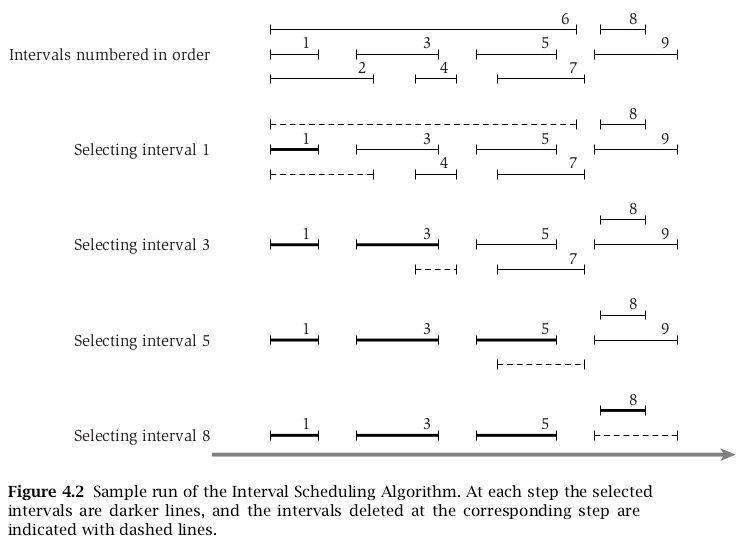
\includegraphics[width=\linewidth]{imagenes/intervalos-compatibles.png}
\end{figure}

\begin{quote}
    De forma inmediata podemos decir que el conjunto retornado tiene request compatibles.
\end{quote}

Lo que necesitamos es demostrar que la solución es optima. Definimos a \(O\), un conjunto de intervalos optimos. 
Luego, vamos a mostrar que \(|A| = |O|\), o sea que el conjunto \(A\) tiene la misma cantidad de intervalos que \(O\), y por lo tanto, \(A\) tambien es una solución optima.

Para la prueba introduciremos la siguiente notación:
\begin{itemize}
    \item Dado \(\{i_1,...,i_k\}\) el conjunto de request en \(A\) en orden que fueron agregados a \(A\). Notar que \(|A|=k\).
    \item Dado \(\{j_1,...,j_m\}\) el conjunto de request en \(O\) ordenos de izquierda a derecha. Notar que \(|O|=m\).
\end{itemize}
El objetivo es probar que \(k=m\).

La manera en que el algoritmo de greedy se mantenga adelante(\textbf{stays ahead}) es que cada uno de sus intervalos finalice al menos tan pronto como lo haga el correspondiente intervalo en el conjunto \(O\).

\begin{figure}[h!]
    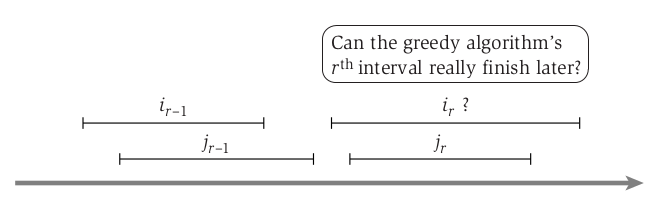
\includegraphics[width=\linewidth]{imagenes/demo-greedy-intervalos.png}
\end{figure}

\begin{quote}
    \textbf{(3.1) Para todos los indices \(r<k\) tenemos que \(f(i_r) \leq f(j_r)\)}
\end{quote}

\textbf{Demostración:}  Probaremos la sentencia anterior mediante el método inductivo. Para \(r=1\) la sentencia anterior es cierta, el algoritmo empieza seleccionando el request \(i_1\) con el menor tiempo de finalización.

Para el caso inductivo, o sea \(r>1\) asumiremos como nuestra hipotesis inductiva que la sentencia es verdadera para \(r-1\), y queremos probar que es tambien es lo es para \(r\). La hipotesis inductiva nos dice que asumamos verdadero que \(f(i_{r-1}) \leq f(j_{r-1})\). Queremos demostrar que \(f(i_{r}) \leq f(j_{r})\).

Dado que \(O\) consiste en intervalos compatibles, sabemos que \(f(j_{r-1}) \leq s(j_r)\). Combinando esto último con la hipotesis inductiva \(f(i_{r-1}) \leq f(j_{r-1})\), obtenemos \(f(i_{r-1}) \leq s(j_{r})\). Asi el intervalo \(j_r\) esta en conjunto \(R\) de los intervalos disponibles al mismo tiempo cuando el algoritmo de greedy selecciona \(i_r\).
El algoritmo de greedy selecciona el intervalo con el \textit{tiempo final mas chico} (\(i_{r}\)); y dado que intervalo \(j_{r}\) es uno de estos intervalos, tenemos que \(f(i_r) \leq f(j_r)\), completando asi el paso inductivo.

De esta forma demostramos que nuestro algoritmo se mantiene adelante del conjunto optimo \(O\). Ahora veremos porque esto implica optimalidad del conjunto \(A\) de algoritmo de greedy.

\begin{quote}
    \textbf{El algoritmo de greedy retorna un conjunto \(A\) óptimo.}
\end{quote}

\textbf{Demostración:} Para demostrarlo utilizaremos la contradicción. Si \(A\) no es optimo, entonces el conjunto \(O\) debe tener mas requests, o sea que tenemos \(m>k\) y aplicando 3.1, cuando r=k, 
obtenemos que \(f(i_k) \leq f(j_k)\). Dado que \(m>k\), existe un request \(j_{k+1}\) en \(O\). Este request empieza despues que el request \(j_k\) termina y por consiguiente despues de que el request \(i_k\) termine.
Entonces, despues de eliminar todos los requests que no son compatibles con los request \(i_1,...,i_k\), el conjunto de posibles requests R aún contiene el requests \(j_{k+1}\). 
Pero el algoritmo de greedy se detiene con el request \(i_k\) y este supuestamente se detiene porque \(R\) esta vacio, lo cual es una contradicción. 



\subsection{Seam Carving - TODO}
Es un algoritmo para adecuar imagenes. Analiza imagenes recortando pixeles de menor importancia. Retira tantas vetas como sea necesario para llegar a un tamaño optimo.


\subsection{Caminimos Minimos - TODO}

Dado dos nodos, uno inicial \(s\) y otro final \(t\) el algoritmo encuentra el camino minimo que los une, tambien entre \(s\) y el resto de los nodos.

\subsection{Compresión de datos - TODO}

El algoritmo de greedy arma un arbol de "hufman" para armar un arbol optimo de prefijos.

\section{División y conquista}

\subsection{Teorema mestro - TODO}


\subsubsection{Mediana con datos separadas}


\section{Programación dinamica}

\subsubsection{Cambio de monedas}

Contamos con un conjunto de monedas de diferente denominación sin restricción de cantidad. Representamos de esta manera \(\$=(c_1,c_2,....,c_n)\) y tenemos un importe x a dar. 
Concluimos que no existe un algoritmo satisfactorio de greedy para resolver este problema.

Si buscamos la solución por \textbf{fuerza bruta}, se puede armar un arbol de decisión. Por cada moneda posible, se genera un subproblema. 
Entonces el camino a la hoja con menor profundidad es la menor cantidad de monedas a dar. Esto hace que la complejidad sea \(O(x^n)\).

Analizando el problema anterios se pueden obtener algunas mejoras. Parte de los caminos del arbol son iguales. 
Hay distintas ramas con nodos que tienen el mismo resto, y por lo tanto se puede calcular solo una vez. Este caso de resto igual en varios nodos, lo llamaremos subproblemas.

\textbf{Subproblema}: Calcular el óptimo(OPT) del cambio \(x\) debe usar el mínimo entre los subproblemas \(X - C_j\) para \(j=1...n\).

Cada vez que paso por un subproblema se \(E\) incremente en el \(1\) que es la cantidad de monedas a dar. Que seria: \(1+min\{subprolemas\}\).

Para la solución \textbf{recurrente}, podemos plantear:

    \[
        \left\{ \begin{array}{lcc}
            OPT(x) = 0 &   si  & x = 0 \\
            \\ OPT(x) = 1+min\{OPT(x-C_i)\} &  si & x > 0 \\
            \end{array}
        \right.
    \]

El resultado con el minimo cambio sera OPT(x) y para poder carcularlo, necesito calcular lo \(x-1\) óptimos anterios. 
Para evitar el recalculo, si calculo el optimo de algun resto, lo almaceno para no volver a calcularlo de nuevo.
Ademas en cada subproblema debo analizar \(n\) comparaciones, lo cual impacta en la complejidad.

Para la solución \textbf{iterativa}: TODO

\subsubsection{Publicidad en la carretera}


\subsubsection{Programación de intervalos ponderados}





\end{document}
